%!TeX spellcheck = en_GB
\documentclass[conference]{IEEEtran}
\IEEEoverridecommandlockouts
% The preceding line is only needed to identify funding in the first footnote. If that is unneeded, please comment it out.
\usepackage{cite}
\usepackage{amsmath,amssymb,amsfonts}
\usepackage{algorithmic}
\usepackage{graphicx}
\usepackage{textcomp}
\usepackage{xcolor}

\begin{document}
	
	%refer the presentations/ notaability hints about writing a paper
	
	% describe the protocol for control access (blockchain part)
	%  Related work
	%	-   traditional architectures commenly employed in the IoT access:
	%	   XACML, OAuth, UMA
	%	   Dependency of a central entity
	
	% Our contribution should focus on the interoperability on the shared data, can be solved by BX view-update solution
	% ???receipt??blockchain???????????????
	%data?????
	%dejima??virtual??????
	
	%???????????????????????data????
	
	%??access verification??? ??new authorization latency ?like call-by-need)
	
	% ??????node???????????????
	% ??????????????????????????????
	% ???????????????????????whitelist???????????????????????????????????

\title{Authorized Updates to Distributed Medical Data}

\author{
	\IEEEauthorblockN{%
		Chunmiao Li\textsuperscript{1},
		Yang Cao\textsuperscript{2},
		Zhenjiang Hu\textsuperscript{3},
		Masatoshi Yoshikawa\textsuperscript{4}
	\vspace{1.5ex}
	\IEEEauthorblockA{%
		\textsuperscript{1,\,3}\,National Institute of Informatics, Japan\qquad
		\textsuperscript{2,\,4}\,Kyoto University, Japan \\
		\textsuperscript{1,\,3}\,SOKENDAI (The Graduate University for Advanced Studies), Japan\qquad
		\textsuperscript{3}\,University of Tokyo, Japan
	}
	\vspace{1ex}
	\IEEEauthorblockA{%
		Email:\
		\textsuperscript{1}\,chunmiaoli1993@nii.ac.jp,
		\textsuperscript{2}\,yang@i.kyoto-u.ac.jp,
		\textsuperscript{3}\,hu@nii.ac.jp,
		\textsuperscript{4}\,yoshikawa@i.kyoto-u.ac.jp
	}
}
}

\maketitle

%???a, the, an ???
\begin{abstract}

% From MedRec: (our target problem)
% We recognize  that not all provider records can or should be made available to  patients (i.e. psychotherapy notes, or physician intellectual property) [6], and thus MedRec does not presume to be an automatic content-management system for all of a Physician's output. ?????????shared data?local data?????????
%MedRec does not claim to address the security of individual provider  databases where the record content is stored. ?=> shared ??????peers????? This must still be managed  by the local IT admin. Nor does MedRec attempt to solve the Digital  Rights Management problem. ?data provider can ??????? as view)

\end{abstract}

\begin{IEEEkeywords}
medical data, authorization, update
\end{IEEEkeywords}

\section{Introduction}

Now a lot of medical data are digitalized so as to be stored and accessed conveniently. A medical record is produced after a patient go to see doctor and often resides on the hospital's database. Medical records contain highly sensitive information about patient privacy. HIPPA Privacy Rule  \cite{centers2004hipaa} in the U.S. regulates the use and disclosure of personally identifiable health information to protect patients' privacy. However, it hard to make sure that all medical institutes would follow these rules and they may expose patient privacy deliberately or for profit. Moreover, a patient might visit many hospitals and leave his records scattered \cite{zhang2016secure} in different places, which make it is hard for he to manage his records efficiently. So patient should be provided a platform to manage and review his historical medical data in case of exposure or being tampered. Better communication between patients and doctors can contribute to patient adherence \cite{zolnierek2009physician} and  improved health \cite{street2009does}. In addition to provide data to doctor, patients tend to share their medical data with health experts to help understand some statistics. Many researches has been done to study how medical specialists with different expertise collaborate with each other \cite{fitzpatrick2013review}.  Researchers can identify public hearth risks and then develop a better treatments by analyzing existing medical data \cite{office2015report}. As presented in \cite{chung2018using},  patients and experts can exchange information to develop better plans to satisfy individual routines. Sharing medical data under some constraints could benefit all relating stakeholders such as patients, researchers and doctors. 
% %??????????????/??????????????????
% %?????????????????????revise treatment plan
% %???????????????????????????????????????

To be shared by multiple parties, shared medical data could reside in encrypted format on the trusted cloud. Only authorized stakeholders can access the shared data. Centralized access control might lead to single point of failure and become the bottleneck of sharing system. Some medical data sharing systems \cite{azaria2016medrec,fan2018medblock,xia2017bbds} are proposed to manage authentication based on blockchain\cite{nakamoto2008bitcoin} technology. Being a immutable shared ledger, blockchain can achieve consensus among distributed nodes via proof of work. Encoding the access control logic of medical data into smart contracts\cite{azaria2016medrec} or Chaincode \cite{dubovitskaya2017secure} can prevent unauthorized party to access medical data, which will guarantee data security. Anyone who want to access medical data should be verified permission from blockchain side and their access process will be recorded on blockchain.

However, generally different stakeholders may have different focus on the same medical records. For example, doctors might be more concerned with the clinical data and researchers are interested in mechanism of action, whereas patients care more about the medicine dosage standard. To reduce the size of shared data to improve access efficiency and avoid additional data interference, the complete medical data (data source) might be split into lots of smaller data pieces (data views) which are shared by different parties. Each view can be regenerated from the source. Source and view should satisfy predefined consistency relationship. Different views from one source might have overlapped data. Moreover, each party will have a local complete data and different data pieces to share with others. In this way, shared data are distributed among sharing parties.
%??????????????????

Not only limited to access data, patients or doctors may want to update existing shared data. Although some works \cite{azaria2016medrec} claimed to allow updates on shared medical data, they did not propose any concrete scheme to implement updates and show how to synchronize all sharing parties to keep them still have same shared data after updates.

%But how about read, add, delete shared data?
%Since the shared data just reside in each peer's local database, read the shared data is easily promised.
In this paper, we aim to solve authorized updates issues on distributed shared medical data as stated above. 
%for updates distributed shared medical data
Each participant may have multiple shared data with different peers and keep this shared ones consistent with local complete database. Bidirectional transformations \cite{hu2014validity} (BXs hereafter) can help synchronize them after updates on either one side. For example, we can use \emph{put} function in BX to reflect modifications on shared data to complete data and \emph{get} to reproduce shared data from complete data. 
%For authorization
Moreover,  any operations on the shared data should be conducted after the peer has been authorized. Any modifications on the existing shared data should be updated to all sharing peers immediately. We encodes the sharing peers not pointers to the raw data into smart contracts in case of private data leakage. Each sharing peer will receive the notification from smart contracts after an update on shared data are verified. Then each peer will request the newest data from updater and then use it to update his local complete data. Smart contracts will refuse any further operations on shared data before all sharing peers have pulled the newest data to their local database.

Our contribution are as follow.
\begin{enumerate}
	\item We surveyed existing blockchain-based solutions and clarify their disadvantages, which are presented in Section \ref{related work};
	\item We designed  a decentralized medical data sharing architecture where data reside on owner's local database and metadata are stored on smart contract of  blockchain.
	\item We proposed that the consistency relationship between local complete data and shared data and apply BX to keep consistency after updates;
	\item We discussed the essential components needed for medical data sharing and proposed our solution to build a holistic solution utilizing blockchain to control updates permission.
	
\end{enumerate}

The remainder are organized like this. Section \ref{preli} gives some preliminaries about blockchain and bidirectional transformations. Section \ref{system} sketches our system architecture and provides a case analysis. Section \ref{discuss} discusses more details about our contributions and propose countermeasures against identified threats to our system. Section \ref{related work} compared our work with existing ones to clarify our improvement over them. Section \ref{conclude} concludes and directs our future work.

\section{Preliminary}
\label{preli}

	\subsection{Blockchain}
	Proposed with Bitcoin \cite{nakamoto2008bitcoin} in 2008, blockchain technology has been widely used in many fields. Blockchain provides a solution for data storage, data transfer and consensus protocol in a distributed and decentralized environment. Generally speaking, blockchain is a shared ledger and replicated by all nodes on a distributed network, which records the historical valid transactions in a chronologically chained blocks. The nodes who generate new blocks via a proof-of-work are called miners.
	
	Not only can support the platform of cryptocurrency, blockchain can also be applied to other scenes. Ethereum \cite{wood2014ethereum} extend blockchain with additions such as a built-in Turing-complete programming language so that one can use this scripts (i.e., Ethereum Virtual Machine (EVM) byte codes) to write programs (i.e., smart contracts \footnote{Hyperledger and others still provide platforms to write smart contracts.}) on blockchain. We can just write Solidity \footnote{https://solidity.readthedocs.io/en/v0.5.2/} programs and then it can be compiled to EVM code. Besides the user accounts controlled by private keys like in Bitcoin, the accounts for smart contracts are allowed in Ethereum. Anyone can build decentralized applications which consists of a collection of smart contracts. Once a transaction involving smart contract creation gets confirmed, an address is generated for the contract and later anyone can send transactions to this address for executing the logic on it. A smart contract transaction is enforced when a miner includes it in a new produced block. Other nodes will validate it and re-run contracts if it is valid.
	
	\subsection{Bidirectional transformation}
	The theory of BXs was proposed to synchronize two parts of related information (i.e., source and view).  A BX consists of a pair of forward and backward transformations. A forward transformation (denoted as \emph{get}) extracts elements from the source to build an abstract view, and the backward transformation (denoted as \emph{put}\footnote{\emph{put} is not a simple inverse of \emph{get}. Instead, it accepts the view and the original source as input and produces an updated source as output.}) embeds information of the view back into the source and produces an updated source. This pair of transformations should satisfy the {\em round-tripping} laws (i.e., {\em well-behaveness}) called \emph{PutGet} and \emph{GetPut} properties. 
	\begin{align}
	get (put(\textbf{source}, \textbf{view}))= \textbf{view} \tag {\emph{PutGet}} \\
	put (\textbf{source}, get (\textbf{source})) = \textbf{source} \tag {\emph{GetPut}} 
	\end{align}
	
	Specifically, \emph{GetPut} refers that no extra update should be performed back on the source when there is no change on the view, while \emph{PutGet} hints that \emph{put} should apply all changes on the view to the source so that the view can be regenerated from the updated source by \emph{get}. The most distinguished point of BX is that view can contain only a few part elements of source. Actually, BX stems from the the view update problem in database \cite{bancilhon1981update}, which studies how to translate the updates on a view table to the updates on the relating base (source) table. By designate some consistency between source and view, BX programs can synchronize the source and view and promise that they satisfy the consistency.
	
	One recent big progress towards practical use of BX is the observation that the essence of bidirectional programming is nothing but writing a well-behaved backward transformation (\emph{put})~\cite{hu2014validity, pacheco2014monadic, pacheco2014biflux}, because the corresponding forward transformation can be derived uniquely and freely. A core language, BiGUL~\cite{bigul}, has been developed for putback-based bidirectional programming.
    %refer BIRD
    
\section{System architecture}
\label{system}
     We are ready to illustrate our system architecture in this section. Part A describes the data \footnote{
	 In our prototype, medical data are entered directly by nodes such as doctor. Later we may consider to use the data from wearable devices.} distribution between sharing peers. Part B presents our system design and later explain it using an update scenario.

\subsection{Data distribution}

% If we build a big contract which is a list of list and each small list is a contract for a shared data

Shared data can exist in different peers, as shown in Fig. \ref{DB architecture}. Suppose there are three entities, doctor, researcher and patient. Doctor and Researcher share some data which are stored in D12 on Doctor side and D21 on researcher side respectively. D12 and D21 should contain the same data, which means if doctor or researcher update this shared data on their own side, then this modification should be propagated to the shared part on the other side. Accordingly, D13 and D31 have the same content and so do in D23 and D32.

Each node will store its all data on a bigger database, such as D1, D2 and D3. Each shared data can be seen as a view which is produced by this bigger database named as source. For example, D12 can be made from D1 by using \emph{get}. If D12 is modified, then the D1 need to be reproduced from original D1 and D12 by using \emph{put}. We just write BX in researcher and patient side to express the pair of \emph{get} and \emph{put} functions.

Note in our data distribution, shared data between any two parties will not be exposed to the third party, which can keep privacy between two parties in some degree. For example, any update on D12 and D21 can only be known by patient and researcher. However, after the change on D21 are reflected to D2, since D2 has been modified, D23 might need to be updated to a new version by using \emph{put} on D2.
%??????????????????????????????????????BX??

Fig. \ref{dataRepresentation} presents an example to show data distribution between patient Alice, doctor Bob and researcher Charlie. Each party have their own local base table, named as D1, D2, D3 respectively. For each table, there are some attributes such as medication name and address on D1. Table D13 (also D31) are shared by Alice and Bob and can be produced from either D1 or D3 by \emph{get}. Table D23 (also D32) are shared by Charlie and Bob and can be generated from D2 or D3 by \emph{get}.  Shared tables all stay in sharing peer's local databases. Note here the metadata collection table resides in the smart contract on blockchain. Each entry of metadata collection table corresponds to a shared table. For example, the entry for D13 or D31 declare that it is shared by Alice and Bob and Bob can update all attributes value but Alice can only change the clinical data. The "Latest Update Time" shows when the metadata was changed most recently. Moreover, "Authority to Change Permission allow Bob to change other peers (here just Alice)'s authority so that Alice can update dosage by change the value for "Dosage" attribute to "Bob, Alice".

\begin{figure}[htbp]
	\centerline{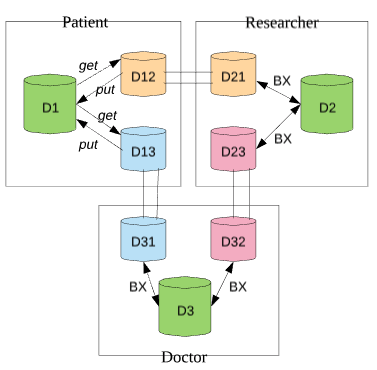
\includegraphics[width=250pt]{DBStructure.png}}
	\caption{DB architecture}
	\label{DB architecture}
\end{figure}

\begin{figure}[htbp]
	\centerline{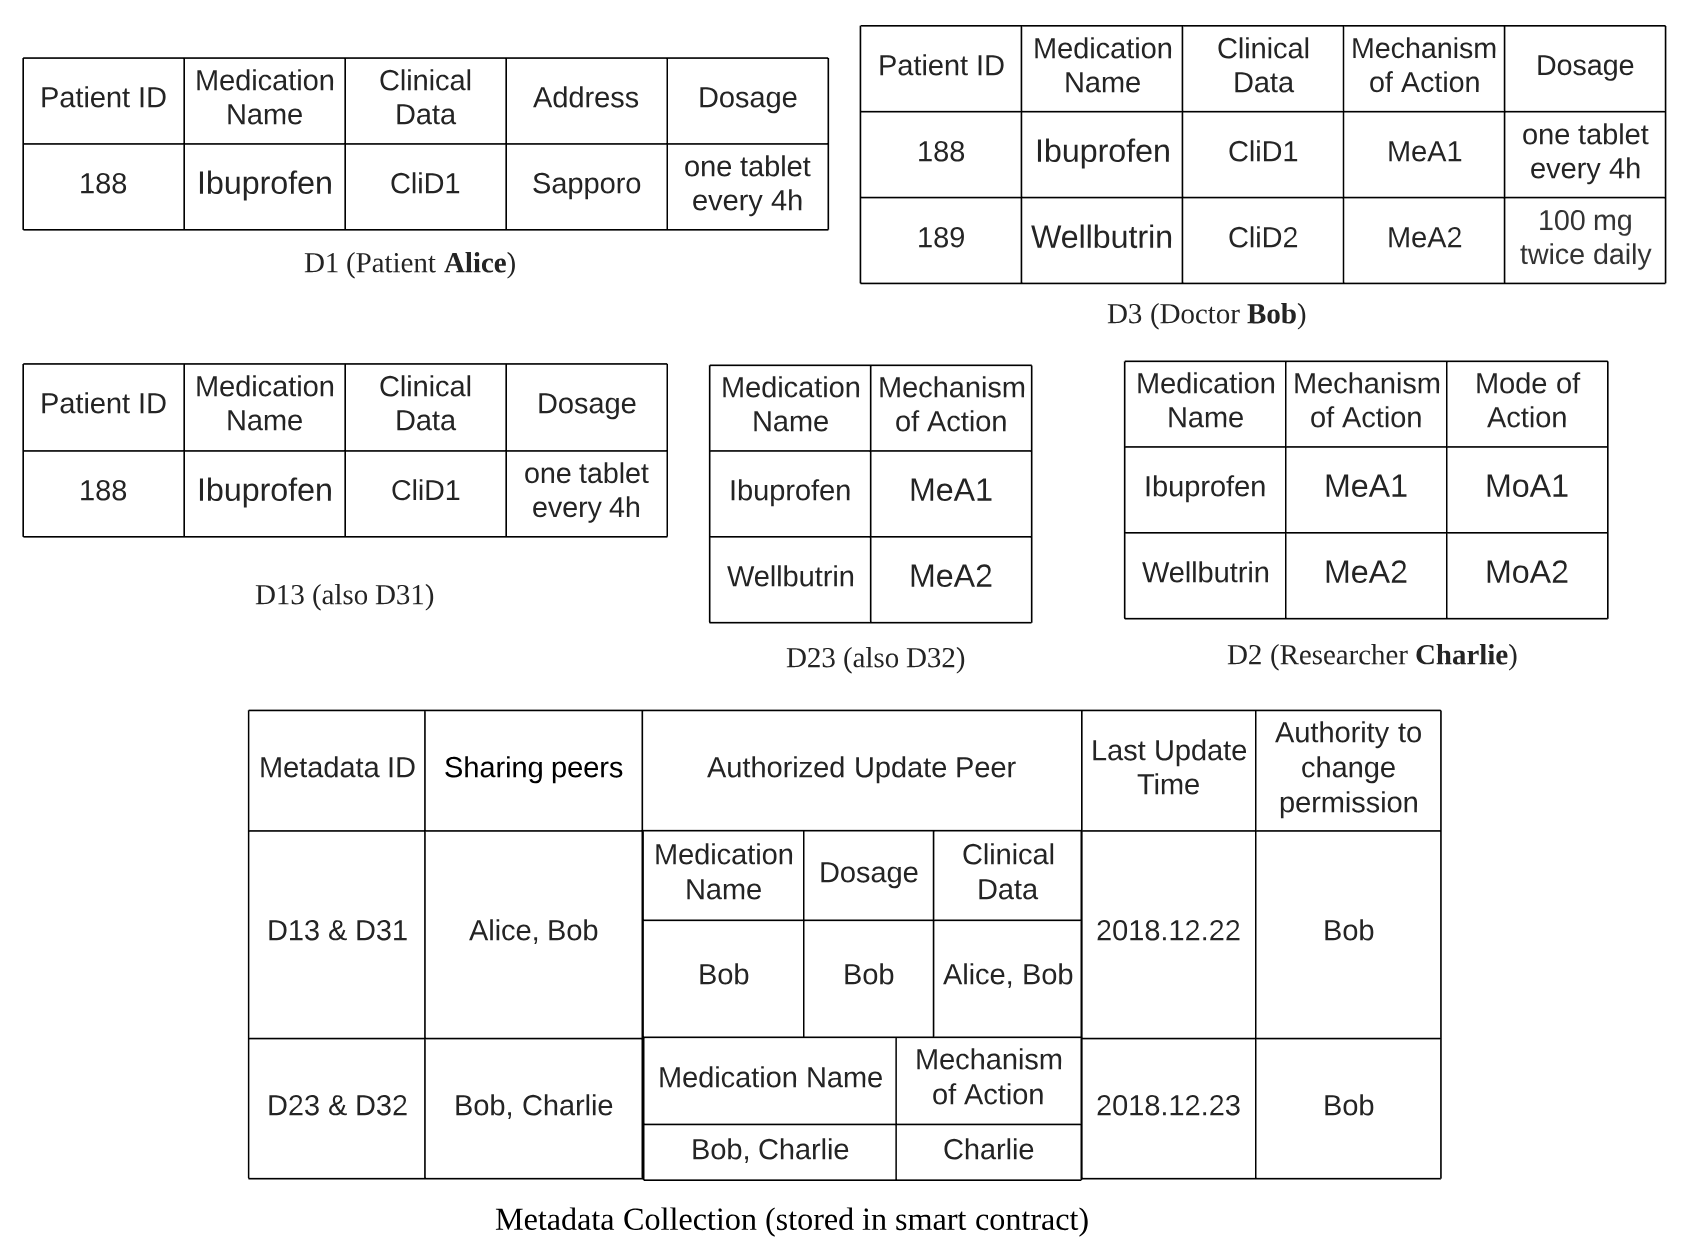
\includegraphics[width=250pt,height=220pt]{medicalData.png}}
	\caption{Data distribution}
	\label{dataRepresentation}
\end{figure}


\subsection{Permission on update data}
The metadata are created immediately once some peers wants to share data with each other. Suppose doctor Bob initiates the data sharing with Alice. He will deploy a smart contract on blockchain which stipulates the metadata about the shared data, such as sharing peers (i.e., Alice and Bob) and so on.  Table Metadata Collection on Fig. \ref{dataRepresentation} are built by Bob. 

Since smart contract can not be altered after it was deployed on blockchain. There are two ways to update the permission for update to shared data:
\begin{enumerate}
	\item deploy a new contract and notify all nodes on blockchain that this new one should be used to verify authority later;
	\item update the state of variables in contract.
\end{enumerate}
We choose the latter way. As shown in Fig. \ref{dataRepresentation}, the authority to modify the update permission are encoded in the field named as "authority to change permission". For example, for D13 and D31, Bob can change the permission to update "Dosage" to "Bob, Alice" so that Patient Alice can also update the  "Dosage".

\subsection{System design}
Our system consists of following components, which can be seen from Fig. \ref{workflow}.
\begin{itemize}
	\item Front-end user interface: control the interaction between users and other components.
	\item Database: each user has an overall database and many shared databases with other users. The latter can always be reproduced from the former.
	\item Blockchain: keep a record of access and update to the shared data. Also, fonrt-end user interface communicate with blockchain network via a blockchain node. The smart contract on blockchain contains the metadata of shared medical data and maintain an update log to store historical modification for each metadata.
	\item Database manager (server) dispose the synchronization between shared data and local data in terms of consistency logic relations.

\end{itemize}

\begin{figure}[htbp]
	\centerline{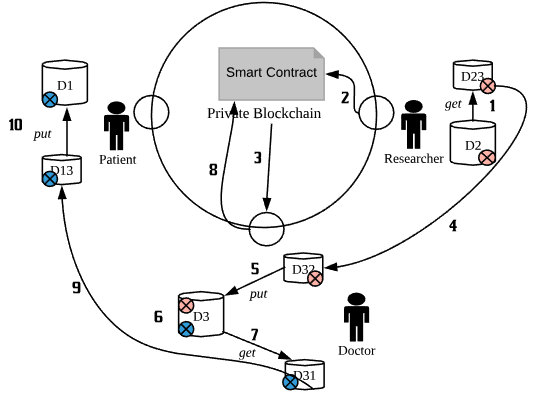
\includegraphics[width=230pt]{updateScenario.png}}
	\caption{An work flow for updating shared data}
	\label{workflow}
\end{figure}

\subsection{Case analysis}
Fig. \ref{workflow} depicts an scenario where researcher initiates the update the shared data. The numbers indicates the corresponding operations sequence.

After the update on D2, the researcher wants to propagate the update to the shared data D23 so that he uses the \emph{put} to regenerate D23 in(step 1). Then he will call a smart contract via a node by sending the repquest for update to the shared data (i.e., D32) (step 2). Note that a smart contract records all permission info about that shared data. Only the researcher's update satisfy the permission can his update be propagated to others. The smart contract will be executed until all nodes form consensus on this update request, which means researcher is authorized to update the shared data with doctor. Each node will conduct the smart contract locally. The metadata of shared data will be updated. Meanwhile, the node relating to Doctor will receive the notification from contract that the shared data with researcher need to modified (step 3). The doctor will request data from researcher by sending a message based on some encrypted communication protocol and get the newest shared data to refresh D32 (step 4). After that, doctor will use \emph{put} to reflect the change on D32 to the total database D3 (step 5). Since doctor shared some data (D31) with patient, he need to check whether D31 need to be reproduced (step 6). If yes, he will use \emph{get} to regenerate D31 (step 7) and request smart contract for permission to update D13 (step 8). Once this permission is allowed, patient will receive the notification about the change on shared data and ask doctor to send the updated D31. After patient get the modified D31 (step 9), he will use this to update D1 via \emph{put} (step 10).  

%Suppose a scenario as follow, which can be seen in Fig....
%
%Suppose Alice, Bob, Charlie are sharing data Da. 
%Alice update the local overall database and want to upload the update on the shared data. She will ask blockchain for permission. After the consensus, she should update the metadata of Da of smart contract on blockchain. Then smart contract will notify Bob and Charlie that the shared data has changed to a new version. Bob and Charlie will send request to Alice. Then Alice will apply \emph{get} to get the view (i.e., updated shared data) and send the Bob and  Charlie the new shared data. Once Bob or Charlie received the new Da, he will update the metadata on smart contract to show that he has upgrade the Da and then use \emph{put} to reflect the change on their own database. 
%
%%here like the orthogonal check on Ominzika sensei's picture
%Next Bob will check whether the update on local big DB will produce a new version of shared data with David. If yes, he will do the same procedure like Alice did at first.
%
%Only Alice, Bob, Charlie received the new Da, then the update on Da is successful. Else rollback???
%
%*************
%
%
%Still Bob need to whether he should update the dejima with David or others 
%
%Dependency 
%Incremental update
%Dependency graph
%
%Just send them data
%Put online; give them link
%Give data to each person
%
%Advantages of having data Locally not on server: 
%fast/easy to access
%Full control own data; change format
%exposed to others (since public available; sensitive data)
%scalability (multi access server; slow)


\section{discussion}
\label{discuss}
In this section, we add more details about our contributions. In addition, we identify some threats to our system and propose relating countermeasures.

\subsection{Detailed contributions}
\begin{itemize}
	\item Nodes can split total data into multiple pieces which can be shared with different nodes, which make sharing exists among only a group of nodes. So that it can avoid the interference or attack from other nodes. Meanwhile, data provider can choose what they want to share with others without exposing sensitive or private information.
	
	\item Any update on shared data can be reflected to local total database by using \emph{put}. Consistency between shared data and local total data are firmly promised by BX. 
	
	\item Permission to updates to medical data are stored in smart contracts so that blockchain can prevent operations from malicious nodes. 
	
	\item Raw medical data always stay in each peer's local database and data transfer only exist between sharing peers, which avoid data being leaked to the third party so as to keep shared data security .
	
	\item Blockchain's  consensus protocol scheme keep the shared data between sharing peers are same after updates since each peer will receive the notification from contracts and pull new shared data from other sharing peers.

	\item Any modification on shared data can be recorded on blockchain. Blockchain properties such as immutability, auditablility and transparency enable nodes to check and review update history on shared data.
	
	\item Simultaneously updates to the same shared data by multiple peers are forbidden. Smart contracts dispose the updates according to received requests in chronological order. If a transaction for updates on shared data has been included in a block, then other requests on this shared data will not be accepted, i.e., one block can contain one transaction at most on some shared data at one time. This can promise that only when all sharing peers have had newest shared data can they execute further operations.
	
	\item Each node can be a shared data provider. As referred in \cite{chung2018using},  many clinics encourage patients to collect data by themselves that are supposed to be gathered by doctors and expect to increase clinic efficiency and promote patient awareness.
	
	\item Our system can also be applied to other scenarios besides medical data sharing.
	
\end{itemize}

\subsection{Threats and countermeasures}
\subsubsection{Throughput}
We employ smart contracts to control access to shared data. As we all known that the block creation time is approximately 12 \textit{s} on Ethereum. We argue that this time interval is acceptable since nodes may choose to collect a lot of updates then send requests to contracts. Usually it is not so urgent for a patient or doctor get the immediate updated shared data.

\subsubsection{Security of smart contracts }
Smart contracts might be the prime targets for attackers. We may apply some theorem prover such as Coq\cite{huet2004coq} to prove or verify the correctness of smart contracts to prevent these attacks.

\subsubsection{Scalability}
Once deployed to the public Ethereum blockchain, transactions relating to our systems might not be chosen into a block by miners. So a private blockchain might be a better choice for our system.

\subsubsection{Incentive}
Like in \cite{dagher2018ancile}, we don't include any incentive for mining beyond the use of our system. We presume that all nodes on the blockchain already have incentives to keep medical data from being tampered and illegal access or updates.

\section{Related work}
\label{related work}
In this section we review existing blockchain-based research on medical data sharing field and state advantages of our system compared with them.

Zyskind et al. suggested using blockchain for access control in \cite{zyskind2015decentralizing} where encrypted data reside on the third party storage. But data might be exposed by this "trusted" third party so that data privacy are violated.

The idea of introducing Blockchain technology to healthcare was presented firstly in \cite{yue2016healthcare} where they use blockchain for data storage to guarantee medical data can not be modified by anyone. Also, they designed a Healthcare Data Gateway (HDG) to control access of the shared data. However, medical data size can become huge so that become a burden for blockchain nodes' storage since each node have the same copy of blockchain. Usually, the size of metadata is smaller than data. (It also depends on the the structure of metadata and data.) We store metadata on smart contracts so as to reduce the storage pressure for each blockchain node.
%Similarly, Patientory \cite{mcfarlane2017patientory} proposed that the medical data is stored directly on the HIPPA-compliant blockchain database.  

MedRec \cite{azaria2016medrec} choose to store raw medical data on providers' database and patients can download the data from it after authorized by smart contract on blockchain. They aimed to enable patient to engage in their healthcare. Whereas in our system, all parties, such as doctors, patients, and researchers can benefit from sharing data with others. MedRec recognized that not all provider data such as physician intellectual property can be exposed to patients \cite{us2017individuals, grossman2011clinical} so that they don't claim to manage contents automatically from physician's output. In our work, instead we allow each node share a piece of medical data not total but still keep consistency between them after the updates to the shared ones. Additionally, any modifications on data shared by two nodes will not be disclosed to the third party which keep the consistency only exists in sharing peers. Moreover, since all shared data with others can be a part of each nodes' local total databases, we can decide whether one shared data have some influence on the other shared pieces and then propagate this change to the third party.

\cite{dubovitskaya2017secure} gave an architecture to mange and share medical data for cancer patient care. They stored encrypted categorized shared data on cloud and relating metadata in blockchain and implemented the prototype on Hyperledger\cite{hyperledger2017hyperledger}. The access control policy are defined in the chaincode Logic by patients. Whereas we think that each data provider not just patients can use smart contracts to encode the control policy when they deploy them to Ethereum. 

Notably, previous three works and others \cite{liu2018bpds,xia2017bbds,amofa2018blockchain,dagher2018ancile,fan2018medblock} mostly targeted to the access problem on shared data but did not pay much attention to updates on the them. Additionally, they presumed that different parties can share the same data. Unlike them, we aims to solve the updates issues on the shared data and allow one party can split total data into multiple pieces (i.e, views) which are shared with different parties but still keep consistency between source and views.


\section{Conclusion}
\label{conclude}

We are still developing our prototype to implement our idea.
In the future, we will use the real patient data to do experiment but use some de-identification technology to protect patient data from being exposed in terms of  

\section*{Acknowledgment}
The authors would like to thank all PRL lab members for their helpful advice in the draft version.  This work was supported by ...

\bibliographystyle{IEEEtran}
\bibliography{ref}

\end{document}
